
\begin{figure}
%\chapter{Appendix}
\label{Appendix}
\section{Screen Shots}
\begin{center}
\scalebox{0.25}
%{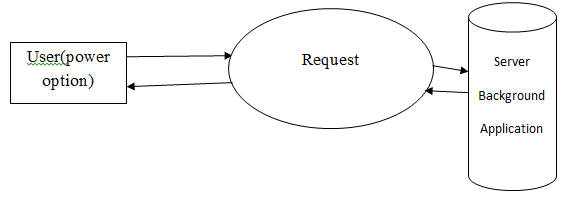
\includegraphics{power1.png}}
{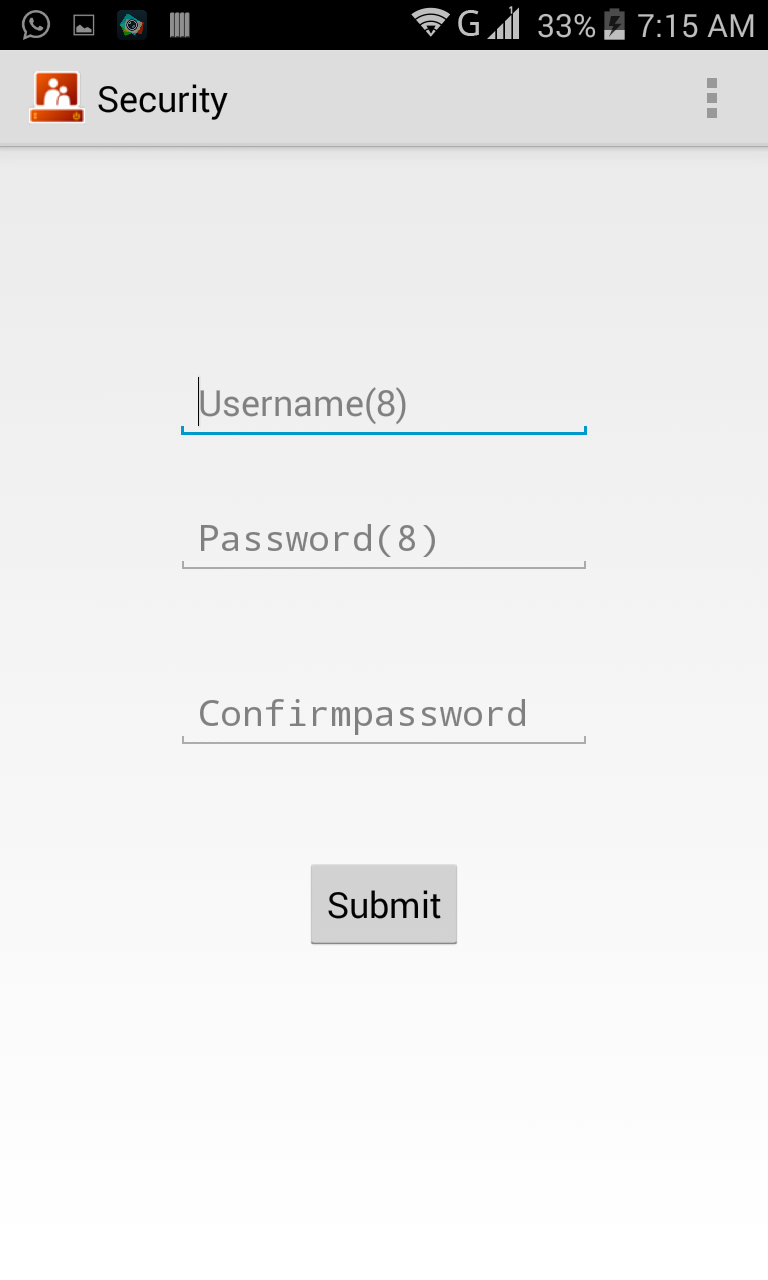
\includegraphics{reg.png}}
\caption{User Registration}  
\end{center}
The mobile user will register in the server database by providing his/her username and password.
\end{figure}

\begin{figure}
\begin{center}
\scalebox{0.25}
%{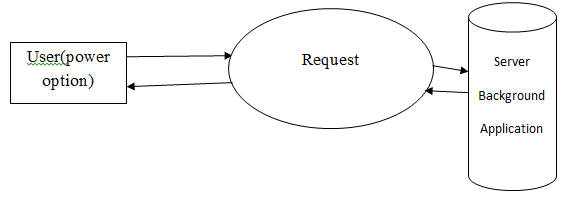
\includegraphics{power1.png}}
{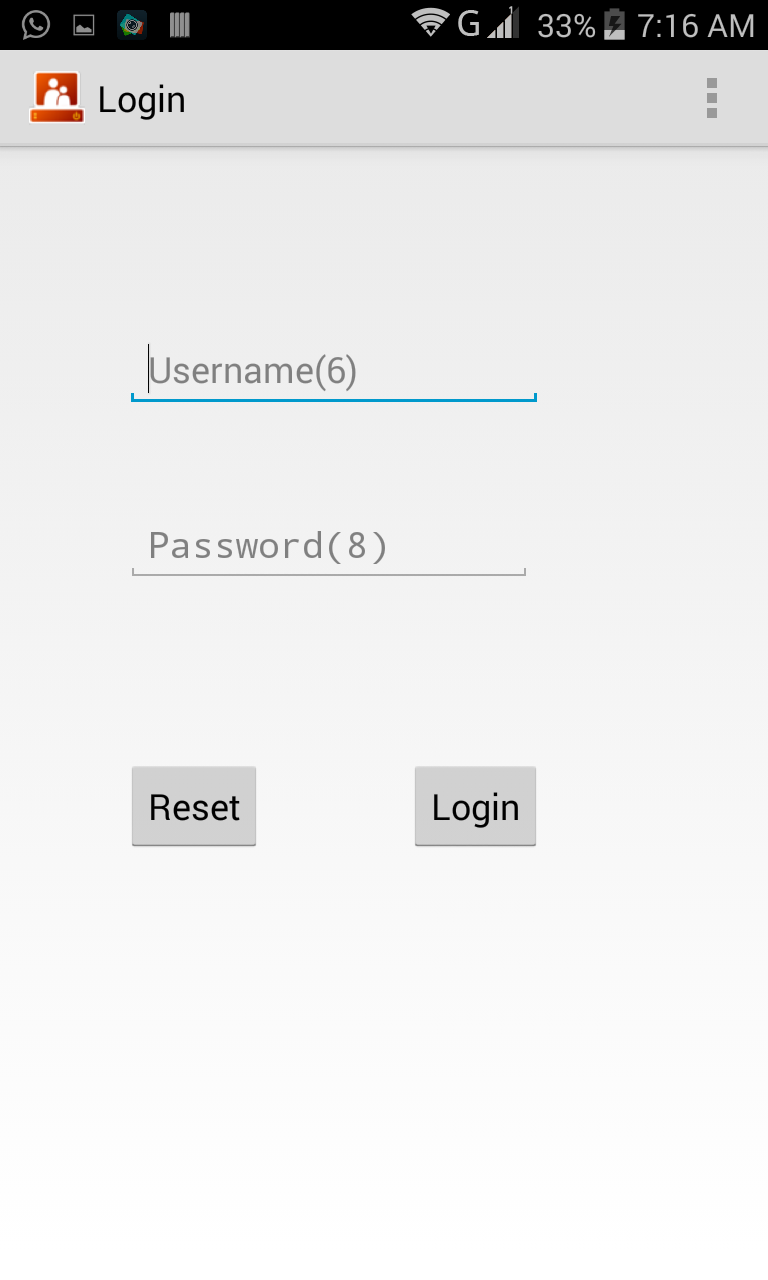
\includegraphics{login.png}}
\caption{User Login}  
\end{center}
The user must complete a login challenge with username and password.
\end{figure}

\begin{figure}
\begin{center}
\scalebox{0.25}
%{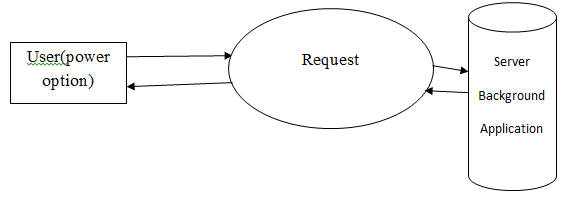
\includegraphics{power1.png}}
{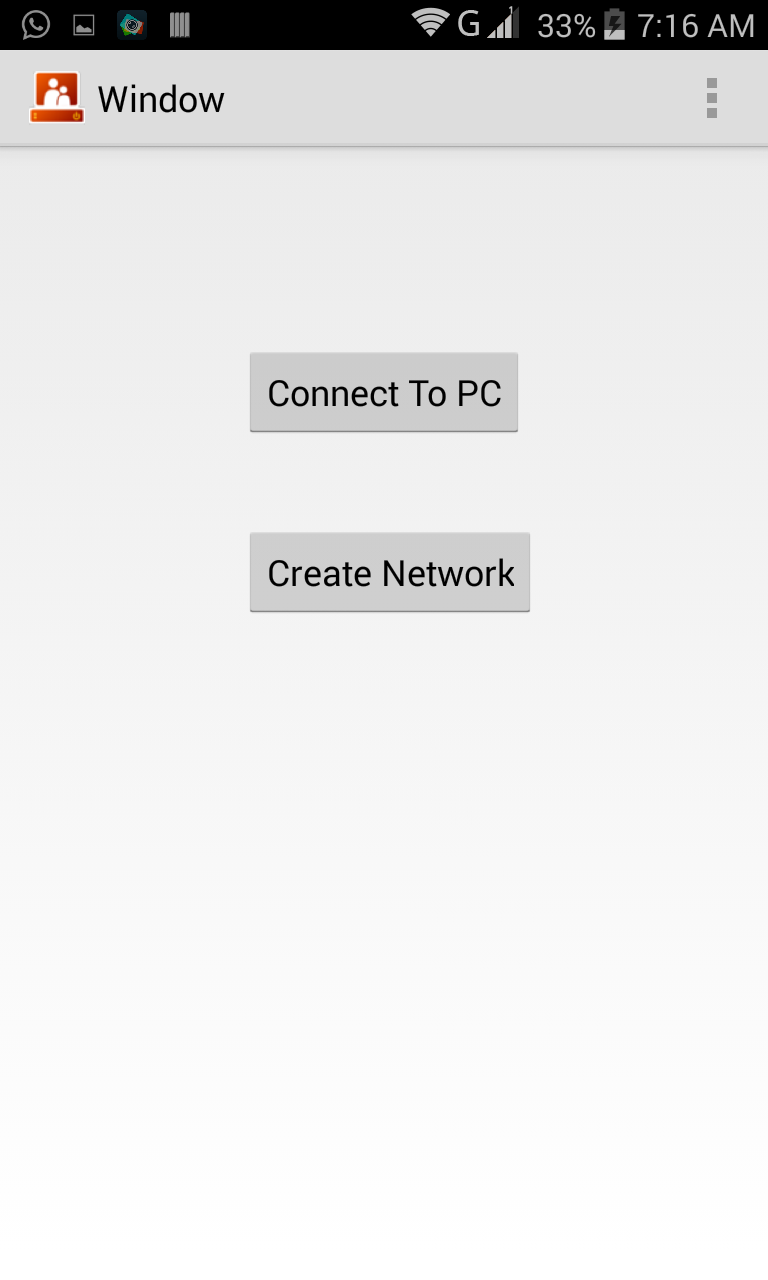
\includegraphics{window.png}}
\caption{Connection Window}  
\end{center}
The connection window contains two options:'Connect to PC' and 'Create Network'. When Create Network option selected control goes to the settings of android and the Connect to PC selected the control goes to the System Configuration. 
\end{figure}

\begin{figure}
\begin{center}
\scalebox{0.25}
%{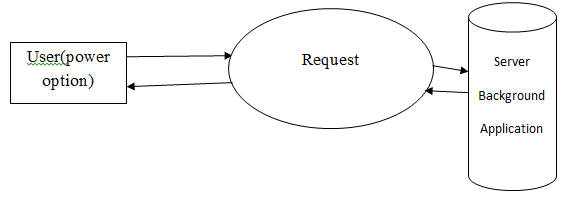
\includegraphics{power1.png}}
{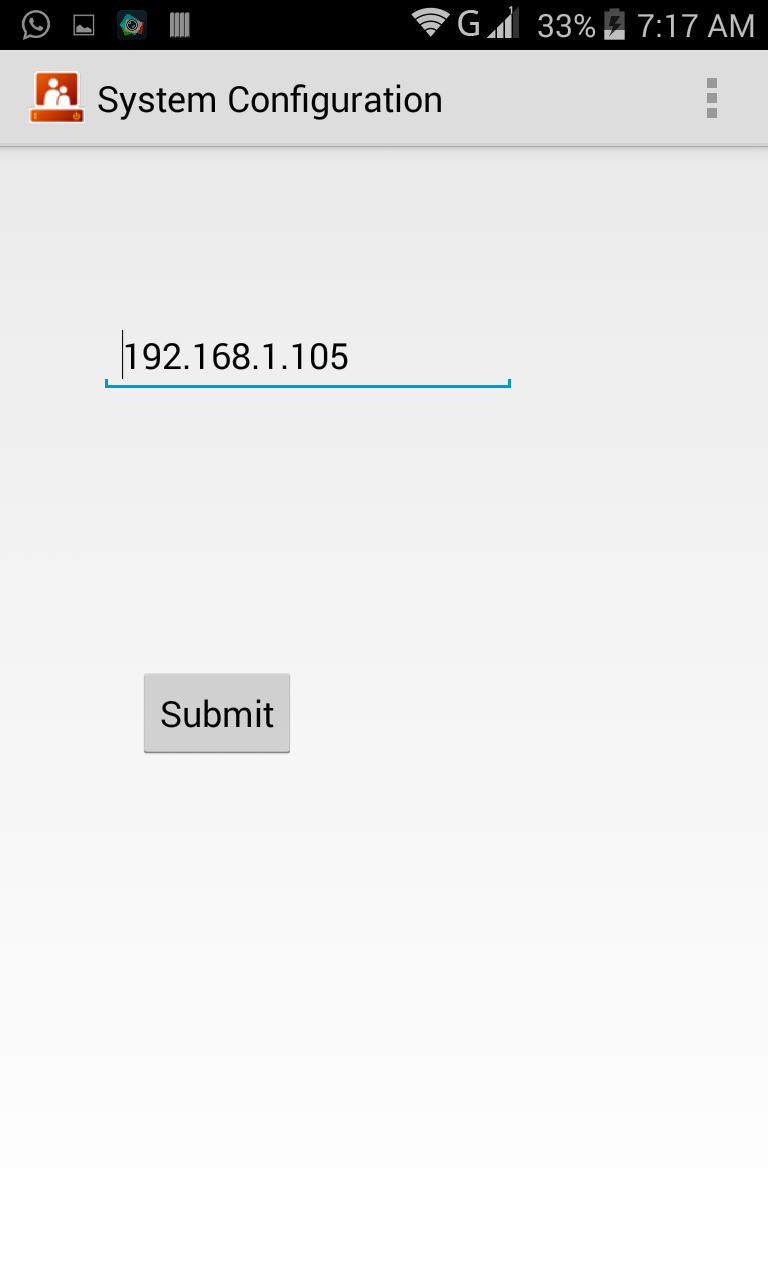
\includegraphics{system.png}}
\caption{System Configuration}  
\end{center}
System Configuration connect the PC to android through IP address. 
\end{figure}

\begin{figure}
\begin{center}
\scalebox{0.25}
%{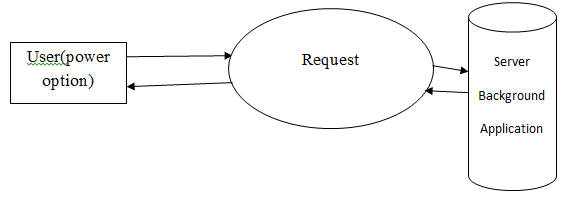
\includegraphics{power1.png}}
{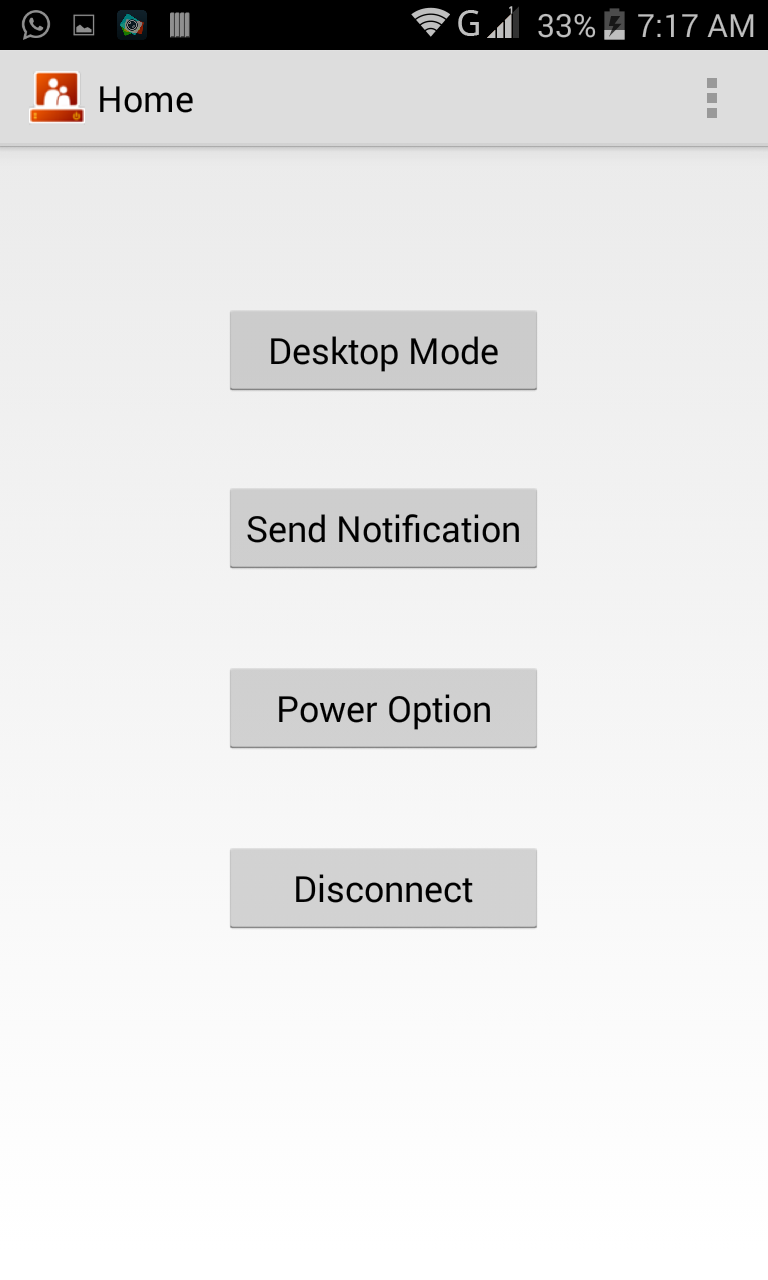
\includegraphics{home.png}}
\caption{Home Options}  
\end{center}
Here four selection options:Desktop Mode, Send Notification, Power Options and Disconnect.
\end{figure}

\begin{figure}
\begin{center}
\scalebox{0.25}
%{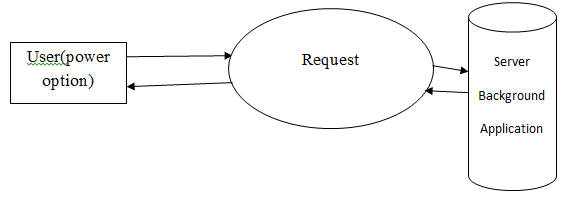
\includegraphics{power1.png}}
{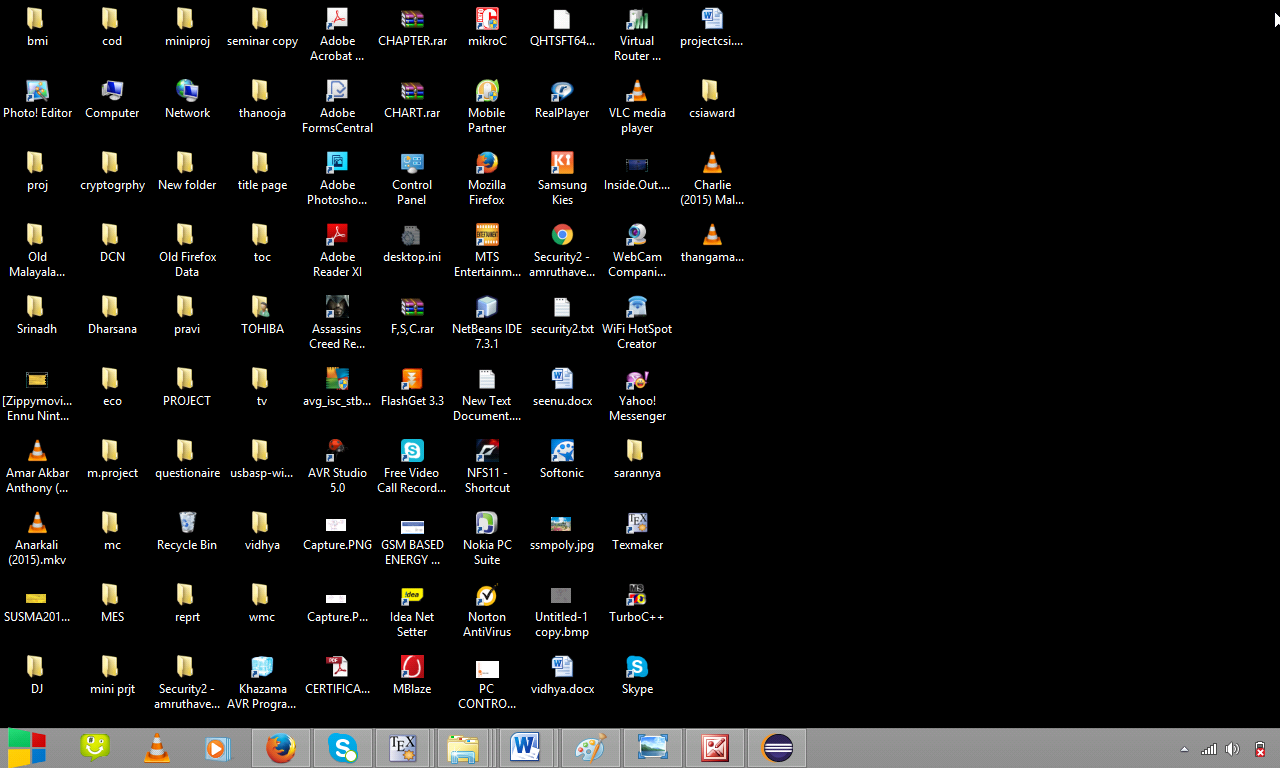
\includegraphics{desk.png}}
\caption{Remote Desktop Access}  
\end{center}
This image shows the desktop of PC in and android.
\end{figure}

\begin{figure}
\begin{center}
\scalebox{0.25}
%{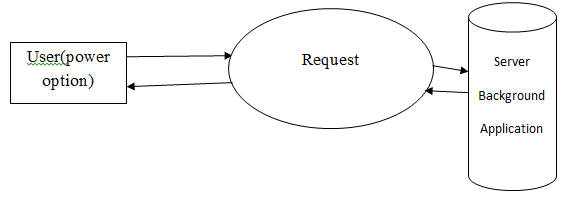
\includegraphics{power1.png}}
{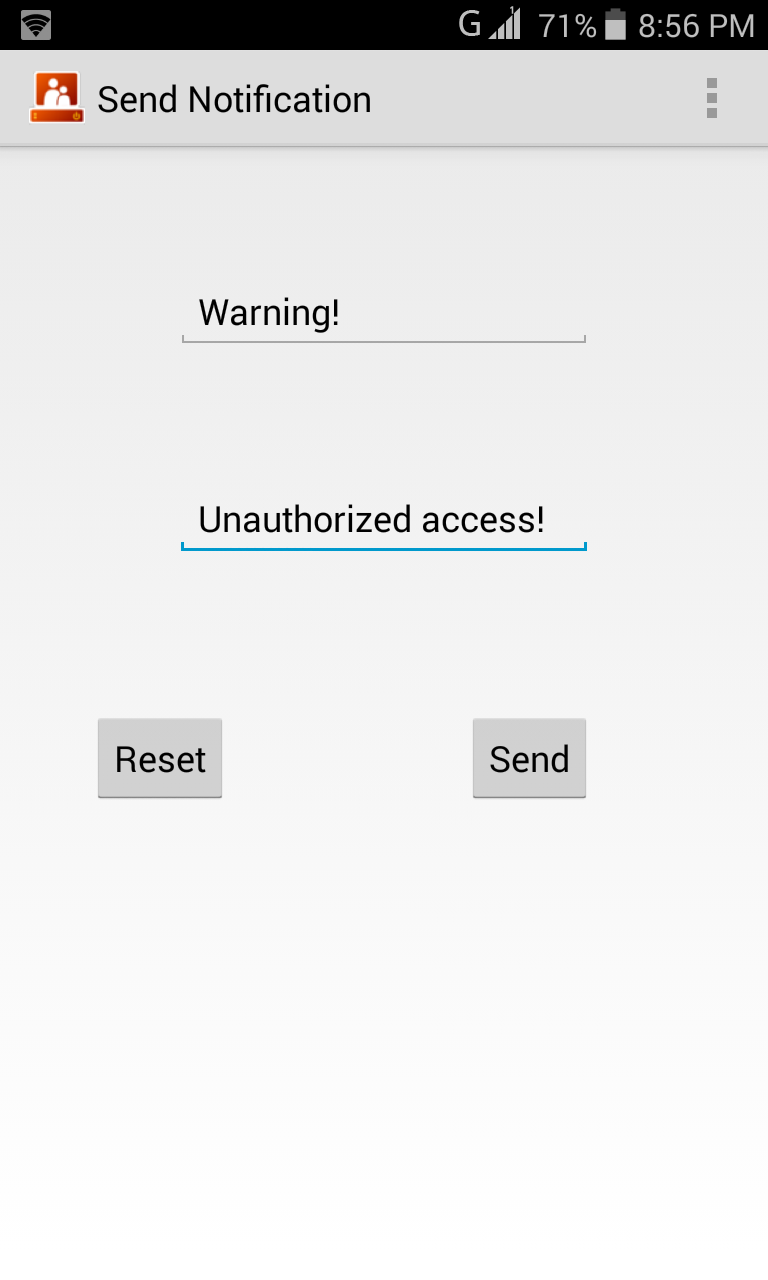
\includegraphics{message.png}}
\caption{Send Notification}  
\end{center}
This window used to send message to the PC.
\end{figure}

\begin{figure}
\begin{center}
\scalebox{0.25}
%{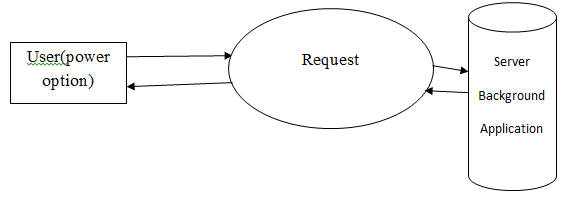
\includegraphics{power1.png}}
{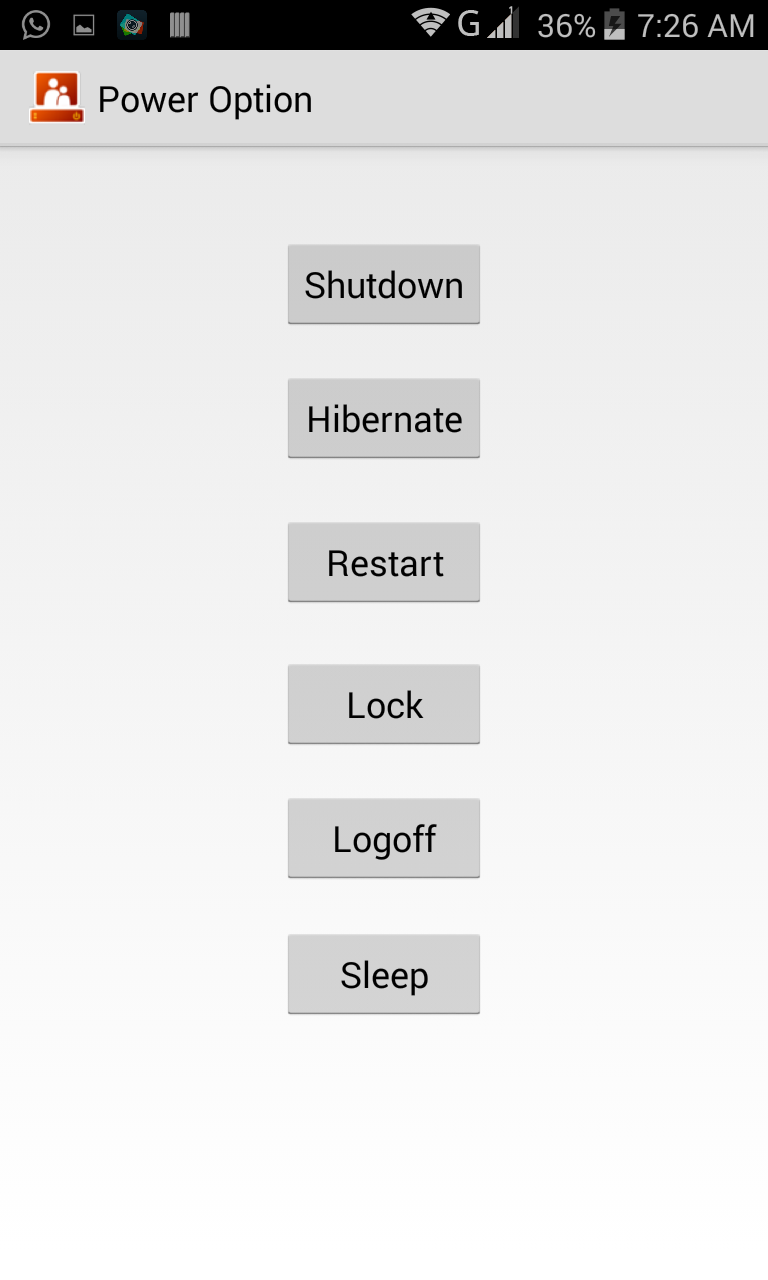
\includegraphics{power.png}}
\caption{Power Options}  
\end{center}
Power option have six selection options. The user can select these options for direct action of Shutdown, Hibernate, Sleep, Restart, Lock, Logoff and Sleep of PC.   
\end{figure}

\begin{figure}
\begin{center}
\scalebox{0.40}
%{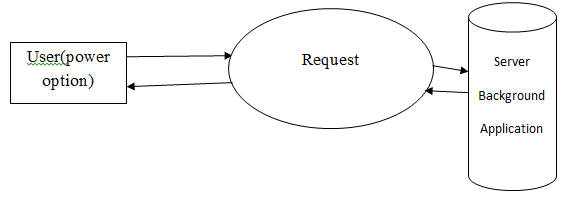
\includegraphics{power1.png}}
{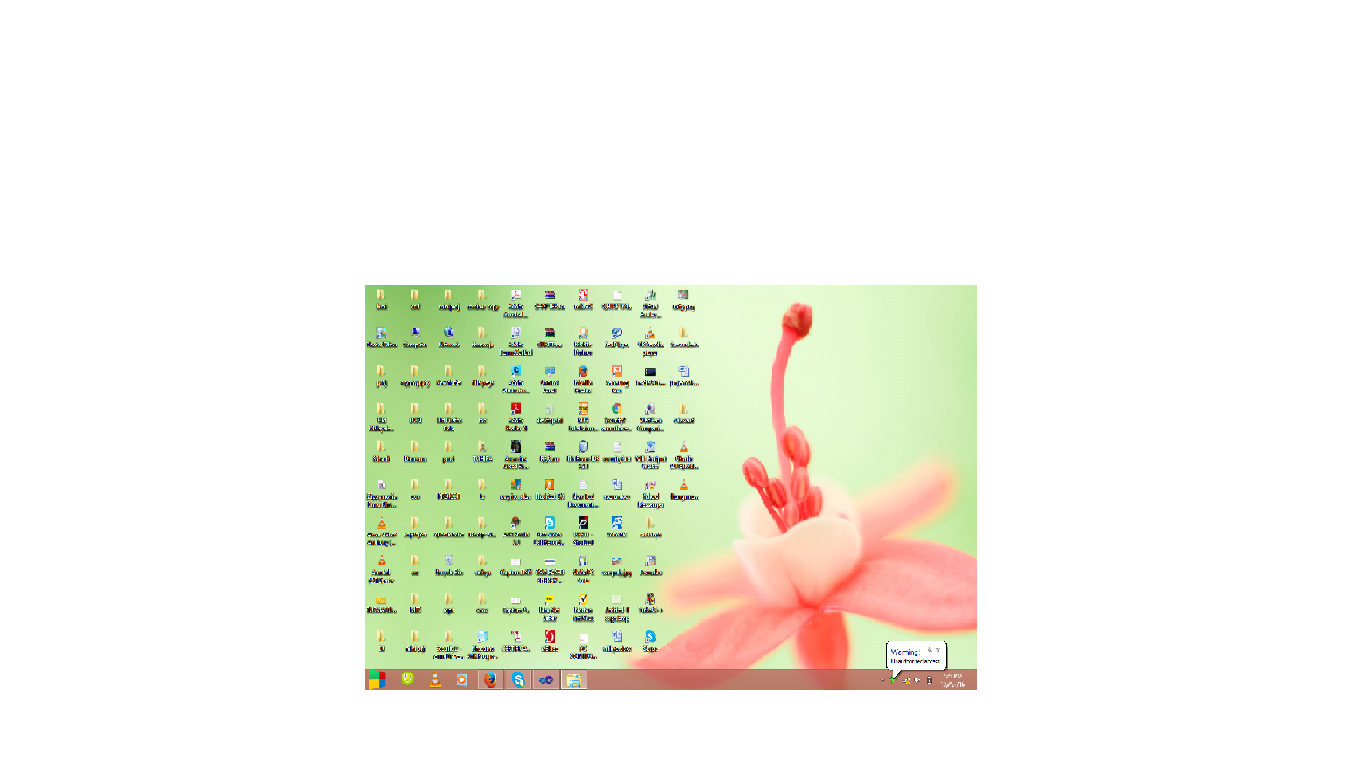
\includegraphics{notify.png}}
\caption{Message Notification}  
\end{center}
This PC desktop image shows the sent message from android.  
\end{figure}

